\section{Corpus y an\'alisis exploratorio}
\label{sec:corpus}

\subsection{Composici\'on}

El corpus de trabajo tiene 169.248 documentos, 34 columnas y 256,9 MB. La Tabla~\ref{tab:composicion} resume la procedencia. La mayor parte viene de rastreo web (104.578) y de Bluesky (64.670). El campo \texttt{source\_type} no sirve como etiqueta sem\'antica: 99.326 filas lo tienen nulo, 64.670 valen \texttt{social\_post} y solo 5.252 valen \texttt{news\_article}. La distribuci\'on por dominio confirma el peso de las fuentes: bsky.app aporta 64.670 documentos, infobae 19.766, eltiempo 12.229, theguardian 7.216 y elespectador 5.456. El corpus no representa la conversaci\'on p\'ublica en espa\~nol: Bluesky llega casi todo en ingl\'es y la prensa est\'a dominada por cuatro cabeceras. La prensa incluye cabeceras brit\'anicas (The Guardian, The Independent, Daily Mail) adem\'as de colombianas (El Tiempo, El Espectador, Infobae).

\begin{table}[t]
\centering
\caption{Composici\'on del corpus por colecci\'on.}
\label{tab:composicion}
\begin{tabular}{lrr}
\toprule
Colecci\'on & Documentos & \% del total \\
\midrule
Rastreo web & 104.578 & 61,8 \\
Bluesky & 64.670 & 38,2 \\
\midrule
Total & 169.248 & 100,0 \\
\bottomrule
\end{tabular}
\end{table}

Tras normalizar el campo \texttt{language}, el corpus queda en 82.682 documentos en ingl\'es, 66.910 en espa\~nol, 13.140 sin idioma declarado y 6.516 en otros idiomas, con 4.133 en h\'ungaro. El h\'ungaro aparece con 4.108 documentos en el campo crudo, un volumen que no corresponde con el resto de la distribuci\'on y que se excluye del filtro de idioma hasta revisarlo. La normalizaci\'on se hace al vuelo en la ingesta y el archivo original no se modifica.

El rango declarado de fechas va de 2008 a 2026, pero 163.736 de los 169.248 documentos (96,7\,\%) no tienen fecha y solo 5.512 la declaran. El filtro temporal se limita a ese 3,3\,\% y as\'i se documenta en la interfaz.

\begin{figure}[t]
\centering
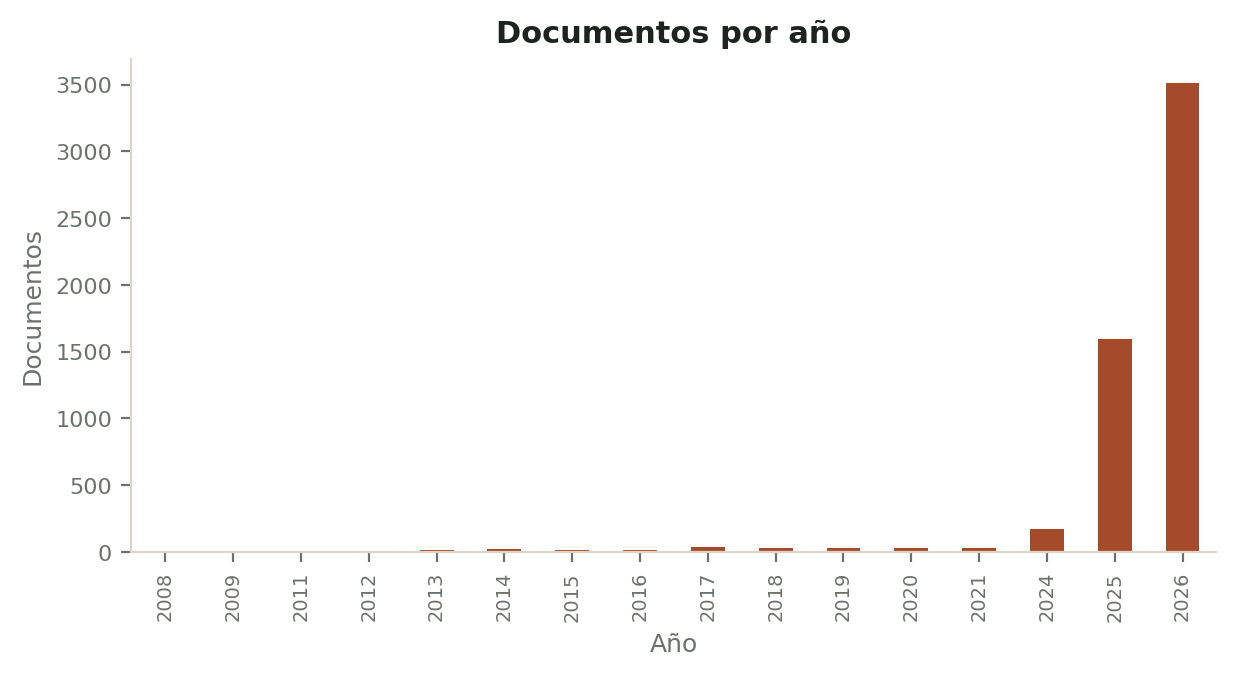
\includegraphics[width=\columnwidth]{perfil_anios.png}
\caption{Documentos por a\~no en el corpus.}
\label{fig:anios}
\end{figure}

\subsection{Duplicados y longitud}

Hay 14.771 copias excedentes (filas que repiten un texto ya presente) agrupadas en 4.434 grupos, con un m\'aximo de 839 copias. Si se cuentan todas las filas que pertenecen a un grupo duplicado, son 19.205: 9.972 en Bluesky y 9.233 en prensa. Las dos cifras son compatibles: la primera cuenta copias adicionales y la segunda, documentos en grupos. No se borran filas en la ingesta, porque eso perder\'ia la procedencia; la deduplicaci\'on se hace en la recuperaci\'on, comparando el hash del fragmento antes de armar el contexto.

La longitud media es de 473 palabras y 2.977 caracteres, pero la mediana baja a 371 palabras y 2.367 caracteres. La cola es larga: el percentil 99 llega a 2.420 palabras y el m\'aximo a 58.181 palabras, equivalentes a 363.528 caracteres. Ese documento extremo produce cientos de fragmentos y obliga a controlar el tama\~no de lote en la ingesta.

\subsection{Ruido de rastreo}

El rastreador dej\'o p\'aginas de error dentro del corpus. La misma p\'agina con los mensajes ``Haz excedido el m\'aximo de peticiones'' y ``Error 505'' aparece en 7.378 documentos, el 4,36\,\% del total, todos en la colecci\'on de prensa. En el conjunto de humo esos textos casi id\'enticos dominaban el top-10 de cualquier consulta, porque su similitud entre s\'i es mayor que la de cualquier documento relevante. El registro de ingesta descarta 7.380 documentos por calidad: 7.378 son esa p\'agina de error y 2 no est\'an desglosados. Quedan 161.868 documentos indexados y 618.286 fragmentos. El porcentaje de documentos con al menos un patr\'on de ruido (peticiones, error 505, cookies, inicio de sesi\'on) llega al 5,3\,\%, pero el filtro solo elimina los marcadores fuertes de error y no las menciones leg\'itimas de cookies.

\subsection{Textometr\'ia}

La textometr\'ia se calcul\'o sobre dos muestras: los 2.000 documentos del piloto y 5.000 documentos estratificados del resto del corpus, con semilla 42. La Tabla~\ref{tab:textometria} compara los indicadores. Los valores son estables entre las dos muestras; eso no demuestra que el piloto represente la distribuci\'on del corpus, solo que no se observan diferencias gruesas en estos indicadores.

\begin{figure*}[t]
\centering
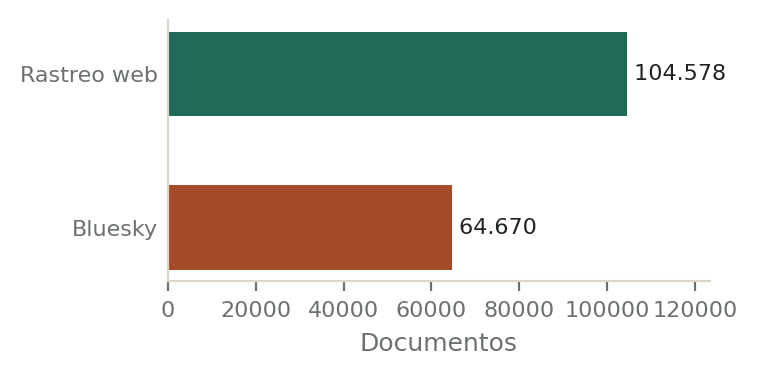
\includegraphics[width=0.8\textwidth]{perfil_colecciones.png}
\caption{Documentos por colecci\'on. Los dos totales coinciden con la Tabla~\ref{tab:composicion}.}
\label{fig:colecciones}
\end{figure*}

\begin{figure*}[t]
\centering
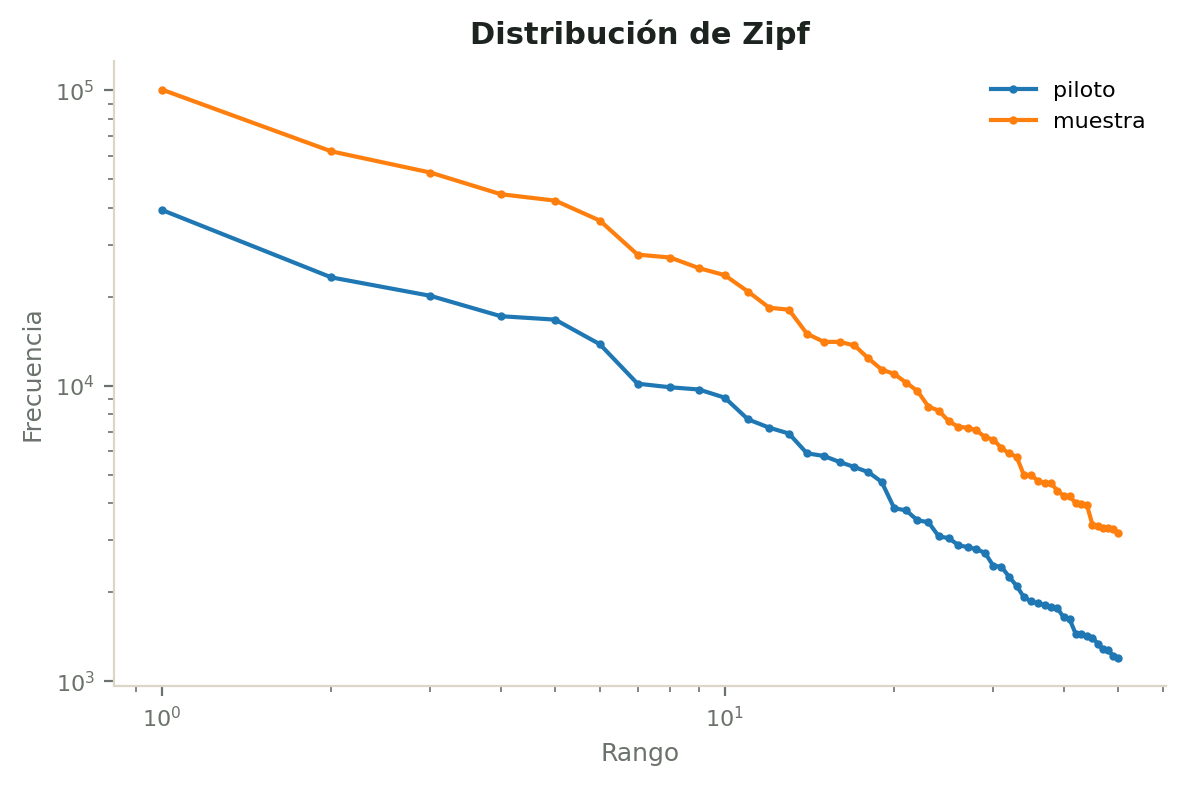
\includegraphics[width=0.8\textwidth]{textometria_zipf.png}
\caption{Rango frente a frecuencia en escala logar\'itmica para el piloto y la muestra. Se muestran los 50 t\'erminos m\'as frecuentes; no se ajusta una recta, la figura solo comprueba la forma de ley de potencia.}
\label{fig:zipf}
\end{figure*}

\begin{figure*}[t]
\centering
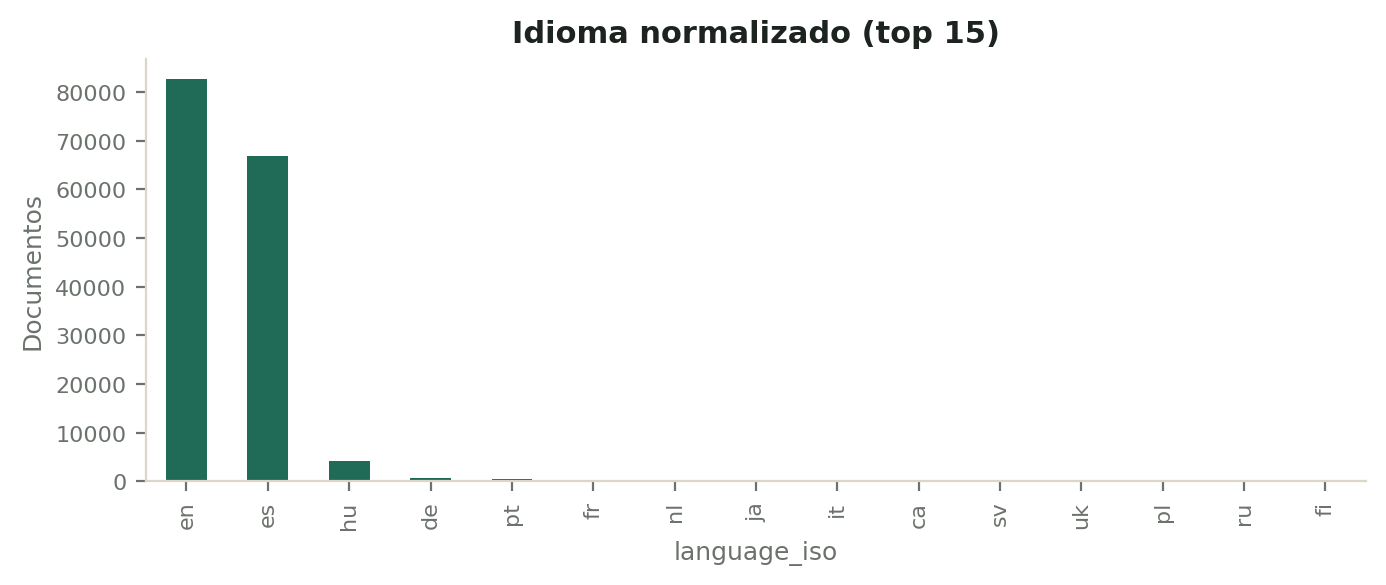
\includegraphics[width=0.8\textwidth]{perfil_idiomas.png}
\caption{Idiomas normalizados m\'as frecuentes (15 primeros). La normalizaci\'on se hace al vuelo; el campo crudo del archivo no se modifica.}
\label{fig:idiomas}
\end{figure*}

\begin{figure*}[t]
\centering
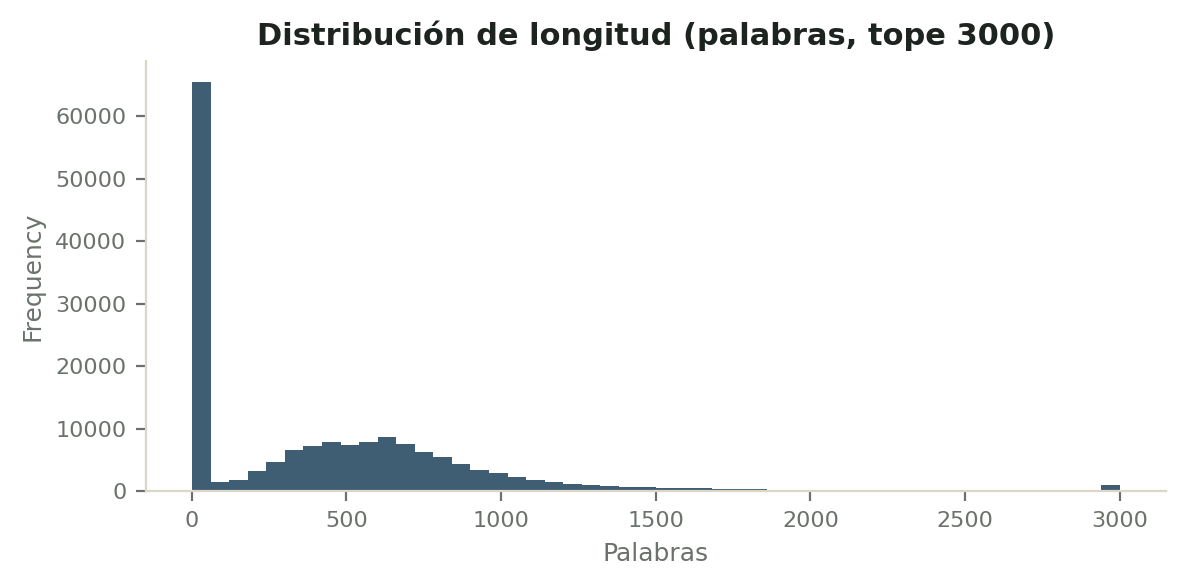
\includegraphics[width=0.8\textwidth]{perfil_longitud.png}
\caption{Distribuci\'on de longitud en palabras. Los documentos de m\'as de 3.000 palabras se acumulan en el extremo derecho del histograma.}
\label{fig:longitud}
\end{figure*}


\begin{table}[t]
\centering
\caption{Textometr\'ia del piloto y de una muestra del corpus completo.}
\label{tab:textometria}
\begin{tabular}{lrr}
\toprule
Indicador & Piloto & Muestra \\
\midrule
Tipos por documento (mediana) & 188 & 188 \\
TTR mediana & 0,579 & 0,570 \\
Hapax / tipos (mediana) & 0,773 & 0,770 \\
Guiraud (mediana) & 10,04 & 10,13 \\
Caracteres por documento (mediana) & 2.317 & 2.353 \\
Caracteres p99 & 14.979 & 15.498 \\
Sin puntuaci\'on terminal (proxy) & 33,5\,\% & 32,7\,\% \\
Documentos con URL & 9,3\,\% & 9,9\,\% \\
Documentos con correo & 1,8\,\% & 1,3\,\% \\
Documentos con emojis & 12,4\,\% & 12,1\,\% \\
Documentos con navegaci\'on & 3,4\,\% & 3,3\,\% \\
Documentos con boilerplate & 3,4\,\% & 4,5\,\% \\
Near-duplicates (SimHash, Hamming $\leq 3$) & 4,25\,\% & 4,72\,\% \\
Grupos de near-duplicates & 26 & 53 \\
Grupo m\'as grande & 12 & 32 \\
\bottomrule
\end{tabular}
\end{table}

El 32,7\,\% de los documentos de la muestra no termina en un signo de cierre. Es un proxy de truncamiento, no una verificaci\'on de que el rastreador los cort\'o: una publicaci\'on completa puede acabar sin punto. La limpieza no puede recuperar ese texto, y el porcentaje se declara como l\'imite en la Secci\'on~\ref{sec:limitaciones}. El HTML residual es marginal (0,14\,\% en la muestra), pero las URLs aparecen en uno de cada diez documentos y los emojis en uno de cada ocho, casi todo en Bluesky. Los near-duplicates no son solo hash exacto: SimHash encuentra grupos de hasta 32 documentos que el hash exacto no captura. Los t\'erminos exclusivos de prensa est\'an dominados por boilerplate (\emph{publicidad}, \emph{informaci\'on}, \emph{adem\'as}), lo que anticipa que una normalizaci\'on conservadora puede ayudar sin destruir entidades.

\begin{figure*}[t]
\centering
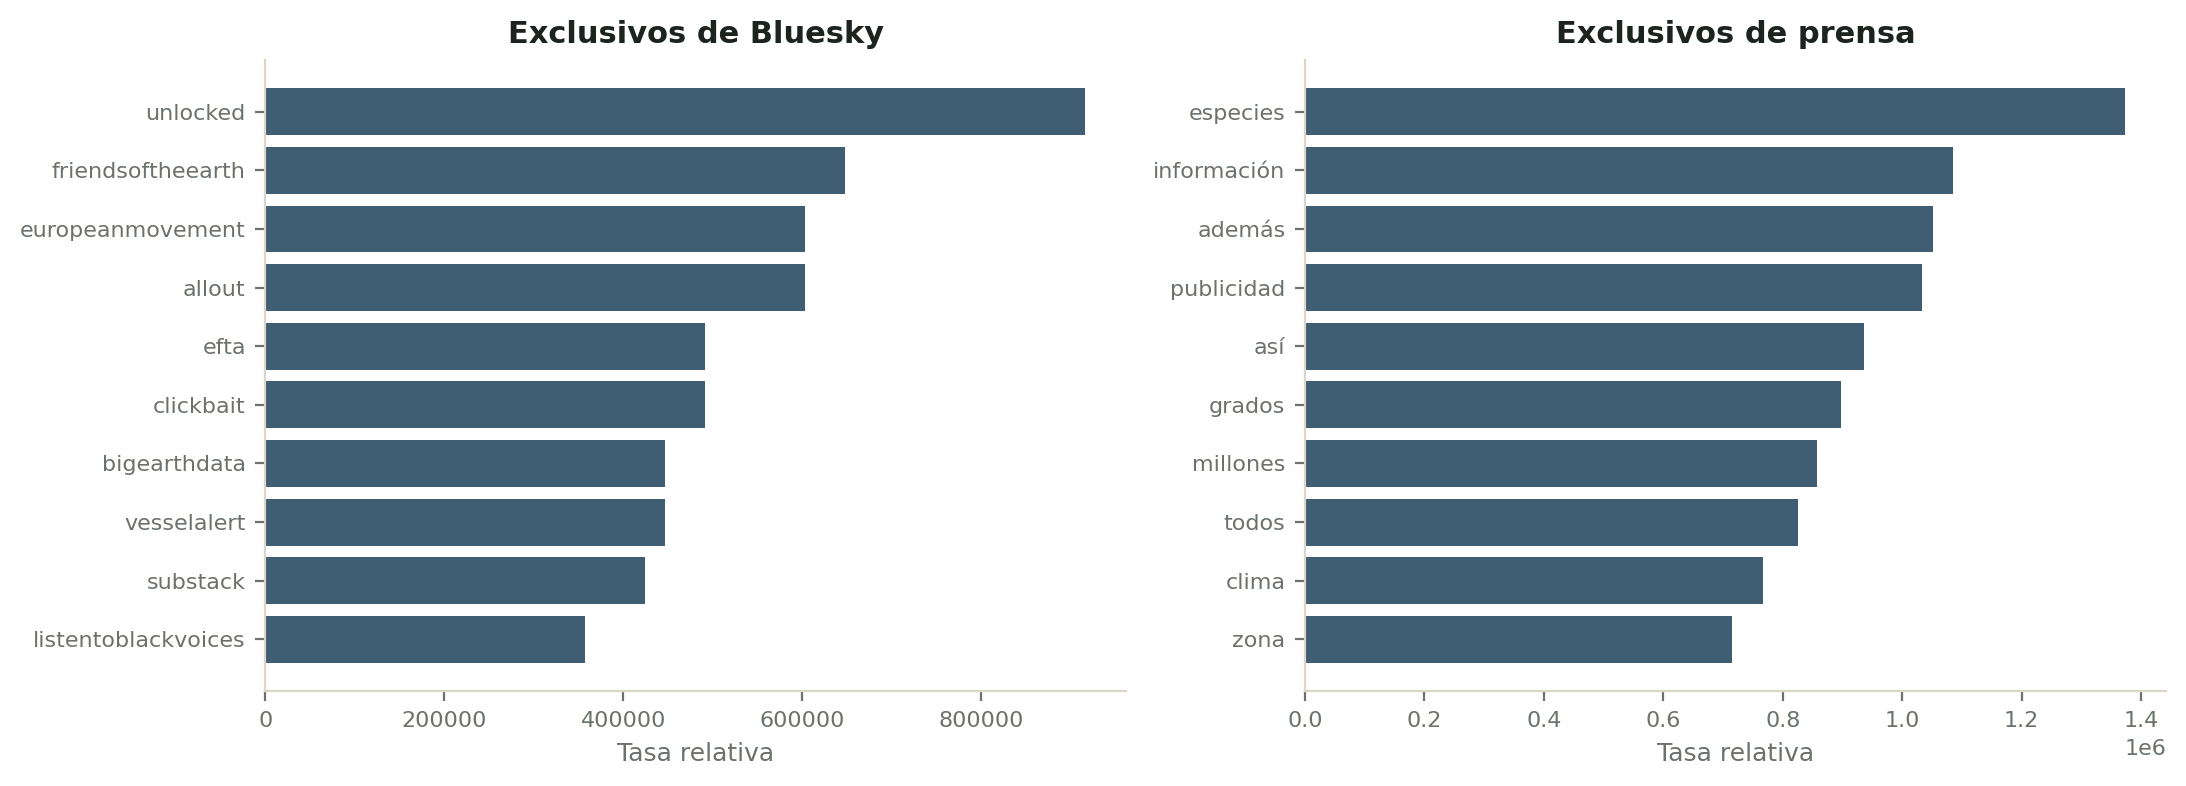
\includegraphics[width=0.8\textwidth]{textometria_terminos.png}
\caption{T\'erminos m\'as frecuentes del piloto y de la muestra.}
\label{fig:terminos}
\end{figure*}

\begin{figure*}[t]
\centering
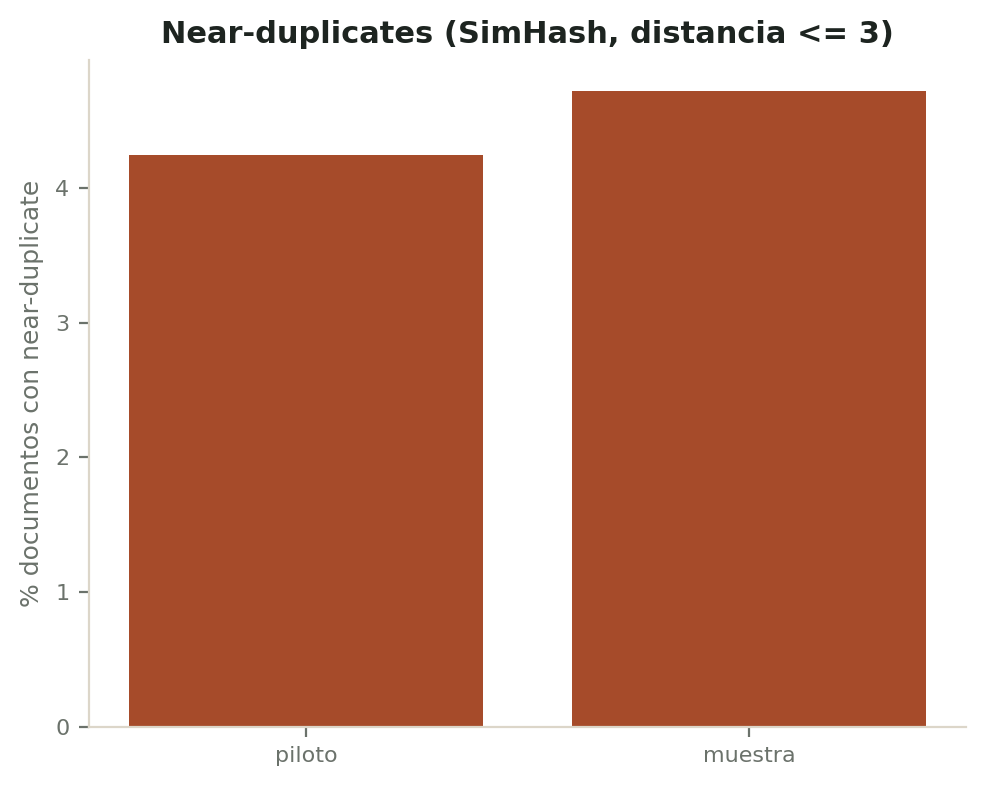
\includegraphics[width=0.8\textwidth]{textometria_near_dups.png}
\caption{Duplicados cercanos: distribuci\'on de similitud entre documentos.}
\label{fig:dups}
\end{figure*}

\begin{figure*}[t]
\centering
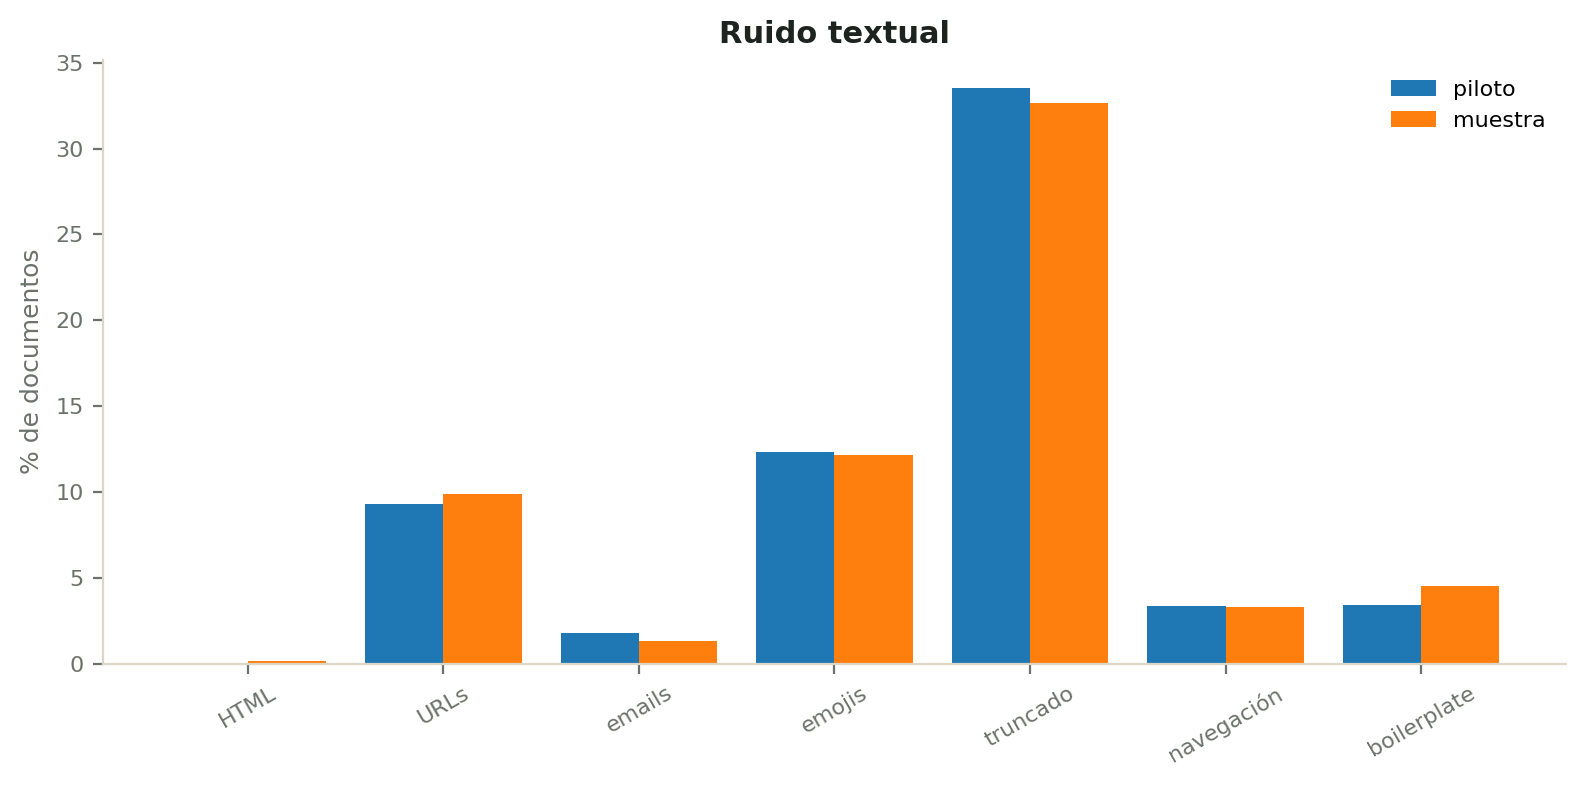
\includegraphics[width=0.8\textwidth]{textometria_ruido.png}
\caption{Indicadores de ruido de rastreo en el corpus.}
\label{fig:ruido}
\end{figure*}

\subsection{Decisiones de procesamiento}

El an\'alisis anterior fija tres decisiones. Primero, limpieza conservadora: se elimina boilerplate y se normalizan espacios, pero no se tocan entidades ni n\'umeros. Segundo, deduplicaci\'on en la recuperaci\'on, no en la ingesta, para conservar la trazabilidad. Tercero, el truncamiento se declara como l\'imite y no se intenta reconstruir. La Secci\'on~\ref{sec:experimentos} mide si la limpieza conservadora mejora la recuperaci\'on frente a no limpiar.
